\documentclass[11pt,a4paper]{article}
\usepackage[T1]{fontenc}
\usepackage[utf8]{inputenc}
\usepackage{lmodern}
\usepackage{amsmath,amssymb,amsthm,mathtools,mathrsfs}
\usepackage{graphicx,float,xcolor,multicol}
\usepackage[shortlabels]{enumitem}
\usepackage[margin=27mm]{geometry}
\usepackage{microtype,needspace,placeins}
\usepackage{tikz,tikz-cd}
\usetikzlibrary{arrows.meta,calc,positioning,patterns,decorations.pathreplacing}
\usepackage[colorlinks=true,linkcolor=teal,urlcolor=teal,citecolor=teal]{hyperref}
\setlength{\parindent}{0pt}
\setlength{\parskip}{.6em}
\setcounter{secnumdepth}{0}
\allowdisplaybreaks
\raggedbottom
\providecommand{\cross}{\times}
\DeclareUnicodeCharacter{2020}{\ensuremath{\dagger}}
\DeclareMathOperator{\supp}{supp}
\DeclareMathOperator*{\esssup}{ess\,sup}
\providecommand{\chapter}{\section}
\newenvironment{tool}[2]{\subsection*{Tool #1 --- #2}}{}
\newcommand{\ToolRef}[1]{Tool #1}
\newcommand{\FigureTag}[2]{\textit{Figure #1}}
\newcommand{\Result}[1]{\subsection*{#1}}
\newcommand{\Application}[1]{\subsubsection*{Application\if\relax\detokenize{#1}\relax\else\space--- #1\fi}}
\newcommand{\ProofHeading}{\par\textit{Proof.}\space}
\newcommand{\ProofOf}[1]{\par\textit{Proof of #1.}\space}
\newcommand{\RemarkHeading}{\par\textbf{Remark.}\space}
\newcommand{\NoteHeading}{\par\textbf{Note.}\space}
\newcommand{\ExerciseHeading}{\par\textbf{Exercise.}\space}

% Rendering support only; mathematical text is in each independent post.
\usepackage{booktabs,array,longtable}
\definecolor{HandoutBlue}{HTML}{2F6690}
\definecolor{HandoutNavy}{HTML}{17365D}
\newtheorem{theorem}{Theorem}
\newtheorem{lemma}[theorem]{Lemma}
\newtheorem{proposition}[theorem]{Proposition}
\newtheorem{corollary}[theorem]{Corollary}
\newtheorem{conjecture}[theorem]{Conjecture}
\newtheorem{definition}{Definition}
\newtheorem{example}{Example}
\newtheorem{namedtoolcounter}{Tool}
\newenvironment{namedtool}[1]{\begin{namedtoolcounter}[#1]}{\end{namedtoolcounter}}
\newtheorem*{claim}{Claim}
\newtheorem*{remark}{Remark}
\newtheorem*{exercise}{Exercise}
\newtheorem*{question}{Question}
\newtheorem*{observation}{Observation}
\newcommand{\SourceChapter}[2]{\section*{#2}}
\newcommand{\Lecture}[2]{\section*{Lecture #1: #2}}
\newcommand{\unclear}[1]{\textit{[unclear: #1]}}
\newcommand{\sourcegap}{\textit{[unfinished in the source]}}
\DeclareMathOperator{\dist}{dist}
\DeclareMathOperator{\id}{id}
\DeclareMathOperator{\Hol}{Hol}
\DeclareMathOperator{\Per}{Per}
\DeclareMathOperator{\Fix}{Fix}
\DeclareMathOperator{\diam}{diam}
\DeclareMathOperator{\Var}{Var}
\DeclareMathOperator{\Leb}{Leb}
\DeclareMathOperator{\Hom}{Hom}
\DeclareMathOperator{\End}{End}
\DeclareMathOperator{\Ann}{Ann}
\DeclareMathOperator{\Spec}{Spec}
\DeclareMathOperator{\Max}{Max}
\DeclareMathOperator{\Ob}{Ob}
\DeclareMathOperator{\Tor}{Tor}
\DeclareMathOperator{\Ass}{Ass}
\DeclareMathOperator{\Mor}{Mor}
\DeclareMathOperator{\Fun}{Fun}
\DeclareMathOperator{\Nat}{Nat}
\DeclareMathOperator{\Cone}{Cone}
\DeclareMathOperator{\MCG}{MCG}
\DeclareMathOperator{\Aut}{Aut}
\DeclareMathOperator{\Deck}{Deck}
\DeclareMathOperator{\SL}{SL}
\DeclareMathOperator{\PSL}{PSL}
\DeclareMathOperator{\Area}{Area}
\DeclareMathOperator{\im}{im}
\DeclareMathOperator{\PSh}{PSh}
\newcommand{\CRing}{\mathsf{CRings}}
\newcommand{\AMod}{A\text{-}\mathsf{Mod}}
\newcommand{\Ab}{\mathsf{Ab}}
\newcommand{\Z}{\mathbb Z}
\newcommand{\Q}{\mathbb Q}
\newcommand{\R}{\mathbb R}
\newcommand{\C}{\mathbb C}
\newcommand{\N}{\mathbb N}
\newcommand{\kk}{\mathbb k}
\renewcommand{\aa}{\mathfrak a}
\newcommand{\bb}{\mathfrak b}
\newcommand{\pp}{\mathfrak p}
\newcommand{\qq}{\mathfrak q}
\newcommand{\mm}{\mathfrak m}
\newcommand{\nn}{\mathfrak n}
\newcommand{\rad}{\mathrm r}
\newcommand{\cat}[1]{\mathsf{#1}}
\setcounter{secnumdepth}{0}
\allowdisplaybreaks

\graphicspath{{figures/commutative-algebra/}}
\begin{document}
\section*{Rings, Ideals, and Prime Ideals}
% BLOG-CONTENT-BEGIN
We shall begin this venture by understanding two fundamental objects: rings and modules.
\subsection{Rings and ideals}
\setcounter{definition}{0}\begin{definition}
A ring $R$ satisfies the following conditions:
\begin{enumerate}[label=(\roman*)]
\setcounter{enumi}{0}\item $(R,+)$ is an abelian group.
\setcounter{enumi}{1}\item For all $x,y,z\in R$, $(xy)z=x(yz)$, $x(y+z)=xy+xz$, and $(y+z)x=yx+zx$ (associativity and distributivity).
\setcounter{enumi}{2}\item $xy=yx$ (commutativity).
\setcounter{enumi}{3}\item There exists $1\in R$ such that $1x=x1=x$ (identity).
\end{enumerate}
If $S\subseteq R$ satisfies (i)--(iv), then $S$ is a \emph{subring} of $R$.
\end{definition}
\setcounter{example}{0}\begin{example}
\begin{enumerate}[label=(\roman*)]
\setcounter{enumi}{0}\item $(\Z,+,\times)$, the ring of integers.
\setcounter{enumi}{1}\item $(\kk,+,\times)$, a field.
\setcounter{enumi}{3}\item $(\kk[x_1,\ldots,x_n],+,\times)$, the ring of polynomials over $\kk$.
\setcounter{enumi}{4}\item $(\{0\},+,\times)$, the zero ring.
\end{enumerate}
\end{example}
% Source page 3
\setcounter{example}{1}\begin{example}
\begin{enumerate}[label=(\roman*)]
\setcounter{enumi}{0}\item $\Z\hookrightarrow\Q$, the field of rationals.
\setcounter{enumi}{1}\item For $P\in\kk^n$, the evaluation map $\kk[x_1,\ldots,x_n]\to\kk$, $f\mapsto f(P)$, is a ring homomorphism.
\setcounter{enumi}{2}\item If $f:A\to B$ and $g:B\to C$ are ring homomorphisms, then $g\circ f:A\to C$ is a ring homomorphism.
\end{enumerate}
\end{example}
\begin{remark}
Denote by $\CRing$ the category of commutative rings. Then:
\begin{enumerate}[label=(\roman*)]
\setcounter{enumi}{0}\item $\Z$ is an \emph{initial object} of $\CRing$: for $A\in\Ob(\CRing)$ there exists a unique $f:\Z\to A$.
\setcounter{enumi}{1}\item $\{0\}$ is the \emph{final object}: for a given $A$ there exists a unique $g:A\to\{0\}$.
\setcounter{enumi}{2}\item If $\{A_i\}_{i=1}^n\subseteq\Ob(\CRing)$, then there exists $A\in\Ob(\CRing)$, called the \emph{product},
\[
A=\prod_{i=1}^n A_i,
\]
with pointwise addition and multiplication, and $(1,\ldots,1)$ as identity. It comes equipped with projections $P_i:A\to A_i$.
\end{enumerate}
\end{remark}
\setcounter{example}{2}\begin{example}
\begin{enumerate}[label=(\roman*)]
\setcounter{enumi}{0}\item If $f\in\Hom_{\CRing}(A,B)$, then $\ker f$ is an ideal of $A$.
\setcounter{enumi}{1}\item For $a\in A$, $(a):=\{xa\mid x\in A\}$ is an ideal of $A$ generated by $a$. Similarly, for a subset $S\subseteq A$,
\[
(S):=\left\{\sum_{i\in F}x_i y_i\ \middle|\ x_i\in A,\ y_i\in S,\ F\text{ finite}\right\}
\]
is the ideal generated by $S$, that is, the smallest ideal in $A$ containing $S$.
\setcounter{enumi}{2}\item $(0)$ and $(1)$ are the only ideals of $\kk$. Hence, by (i), every morphism $f:\kk\to B$ with $B\ne0$ is injective.
\setcounter{enumi}{3}\item If $\{\aa_i\}_{i\in I}$ are ideals of $A$, then so are
\[
\sum_{i\in I}\aa_i:=\left\{\sum_{i\in F}a_i\ \middle|\ a_i\in\aa_i,\ F\subseteq I\text{ finite}\right\},
\qquad \bigcap_{i\in I}\aa_i,
\]
and $\prod_{i\in F}\aa_i$, the ideal generated by $\{\prod_{i\in F}a_i\mid a_i\in\aa_i\}$,
% Source page 6
where $F\subseteq I$ is finite.
\setcounter{enumi}{4}\item In $\Z$, all ideals are of the form $(n)$.
\setcounter{enumi}{5}\item If $\aa,\bb$ are ideals of $A$, then so is the \emph{ideal quotient}
\[
(\aa:\bb):=\{x\in A\mid x\bb\subseteq\aa\}.
\]
If $\aa=(0)$, then $(0:\bb)=:\Ann(\bb)$ is called the \emph{annihilator} of $\bb$.
\setcounter{enumi}{7}\item Let $\aa$ be an ideal of $A$ and $\bb$ an ideal of $B$. For $f\in\Hom_{\CRing}(A,B)$, the ideal $(f(\aa))$ generated by $f(\aa)$ in $B$ is called the \emph{extension} of $\aa$ to $B$, denoted $\aa^e$. The ideal $f^{-1}(\bb)$ of $A$ is the \emph{contraction} of $\bb$ in $A$, denoted $\bb^c$.
\end{enumerate}
\end{example}
\subsection{Distribution of ideals of \texorpdfstring{$A$}{A}}
\begin{enumerate}[label=(\roman*)]
% Source page 8
\setcounter{enumi}{3}\item If, for an ideal $\pp$ of $A$, $A/\pp$ is an integral domain, then $\pp$ is a \emph{prime ideal}; equivalently, $xy\in\pp\Rightarrow x\in\pp$ or $y\in\pp$.
\end{enumerate}
\setcounter{theorem}{0}\begin{lemma}[Prime avoidance]
If $\{\pp_i\}_{i=1}^n$ are prime ideals and $\aa$ is an ideal with $\aa\subseteq\bigcup_{i=1}^n\pp_i$, then $\aa\subseteq\pp_i$ for some $i$.
\end{lemma}
\setcounter{theorem}{1}\begin{lemma}[Factoring]
If $\{\aa_i\}_{i=1}^n$ are ideals and $\pp$ is a prime ideal such that $\pp\supseteq\bigcap_{i=1}^n\aa_i$, then $\pp\supseteq\aa_i$ for some $i$.
\end{lemma}
\begin{proof}
If $\aa_i\nsubseteq\pp$ for every $i$, choose $x_i\in\aa_i$ with $x_i\notin\pp$. But $\prod_{i=1}^n x_i\in\bigcap_i\aa_i\subseteq\pp$, a contradiction.
\end{proof}
\begin{remark}
In particular, if $\pp=\bigcap_{i=1}^n\aa_i$, then $\pp=\aa_i$ for some $i$.
\end{remark}
\setcounter{theorem}{2}\begin{proposition}
\[\rad((0))=\bigcap_{\pp\text{ prime}}\pp.\]
\end{proposition}
\begin{proof}
If $f\in\rad((0))$, then $f^n=0\in\pp$, so $f\in\pp$ and hence $f\in\bigcap_{\pp\text{ prime}}\pp$.
If $f\notin\rad((0))$, let $\Sigma$ be the poset of all ideals $\aa$ such that $f^n\notin\aa$ for every $n$. As $0\in\Sigma$, this poset is nonempty. If $\{\aa_i\}_{i\in I}$ is a chain, then $\bigcup_i\aa_i\in\Sigma$ and bounds the chain. By Zorn's lemma, $\Sigma$ has a maximal element $\mm$.
\emph{Claim:} $\mm$ is prime.
% Source page 10
Let $x,y\notin\mm$. Then $\mm+(x),\mm+(y)\notin\Sigma$ by maximality. Therefore, $f^a\in\mm+(x)$ and $f^b\in\mm+(y)$, so $f^{a+b}\in\mm+(xy)$ and thus $xy\notin\mm$. Therefore $f\notin\mm$, implying $f\notin\bigcap_{\pp\text{ prime}}\pp$.
\end{proof}
The following picture summarizes what we have seen thus far.
\begin{figure}[H]\centering
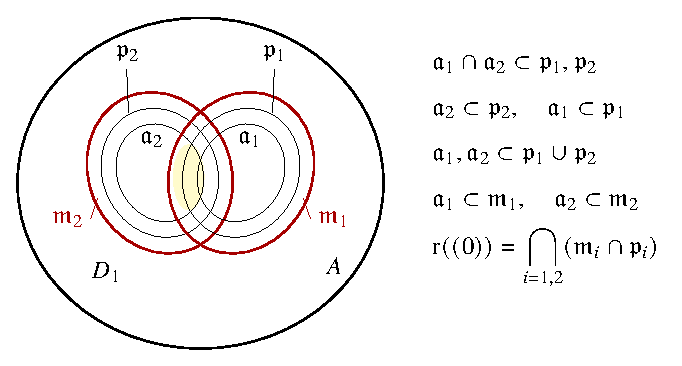
\includegraphics[width=.86\textwidth]{ca1-fig-05.pdf}
\FigureTag{CA1.5}{fig:ca-1-05}
\end{figure}
% BLOG-CONTENT-END
\end{document}
